\section{09. Mai 2012}

\question{Skizzieren der wesentlichen Elemente der Born-Oppenheimer Näherung.}
\label{q:21}

Da die Atomkerne eine wesentlich größere Masse als die Elektronen haben und sich dadurch viel langsamer bewegen, ist es mit der Born-Oppenheimer
Näherung möglich die Positionen der Kerne zu fixieren. Somit lässt sich die molekulare Schrödingergleichung in eine für die Kerne und eine
für die Elektronen aufteilen.

\begin{itemize}
    \item Für die Elektronen stehen die Kerne still, wodurch ihre Lage als Parameter in das anziehende und abstoßende Potential eingeht.
        Somit hängen die elektronischen Eigenzustände und Energien nur von der Lage der Kerne ab und nicht von der Geschwindigkeit.\\
            Die Schrödingergleichung für die Elektronen lautet somit:
            
        \begin{align}
            \hat{H}_e \cdot \Phi_h(\vec{r},\vec{R}) = E_h(\vec{R}) \cdot \Phi_h(\vec{r},\vec{R})
        \end{align}

        Dabei ist $\vec{r}$ die Position der Elektronen und $\vec{R}$ die der Kerne. Der Hamilton-Operator besteht aus $\hat{H}_e = \hat{T}_e + \hat{V}_{ee} + \hat{V}_{eN}$, 
        also der kinetischen Energie der Elektronen + der Abstoßung zwischen den Elektronen + der Anziehung zwischen Kernen und Elektronen.

        \begin{equation}
            \label{eq:electronic_hamiltonian}
            H_{\text{elec}} = - \sum_i \frac{\hbar^2}{2m_e} \nabla^2_i - \sum_{a,i} \frac{Z_a e^2}{4 \pi \epsilon_0 |\vec{r}_i-\vec{r}_a| }  + \sum_{i<j} \frac{e^2}{4 \pi \epsilon_0 |\vec{r}_i-\vec{r}_j| }
        \end{equation}

    \item Die Kernbewegung ist von den Elektronen nahezu unbeeinflusst, jedoch bewegen sie sich im Potential der elektrischen Zustände. 
        Die Kern-Wellenfunktion $\eta_{hk}(\vec{R})$ hängt nur von der Kernkoordinate $\vec{R}$ ab.

        Die Schrödingergleichung lautet:
        \begin{align}
            (\hat{T}_n + \hat{V}_{NN} + E_h(\vec{R})) \cdot \eta_{hk}(\vec{R}) = E_{hk} \cdot \eta_{hk}(\vec{R})
        \end{align}
\end{itemize}



\question{Welche Informationen über molekulare Kerngrößen können aus Rotations-Schwingungsspektren von Molekülen erhalten werden?}
\label{q:22}

(siehe auch \aqref{2}.)

\begin{itemize}
    \item Rotationskonstanten $B_e$ und $\alpha_e$ 
    \item Gleichgewichtsabstand $R_e$
    \item Form der Potentialkurve
\end{itemize}
Die Rotationsenergieniveaus eines Moleküls sind direkt mit dessen Massenverteilung verbunden.
Die Kenntnis der Emissionslinien bzw. Absorbtionslinien (meistens $>\SI{800}{nm}$) ermöglicht es das Trägheitsmoment $I$ des Moleküls zu bestimmen.
\begin{align}
    E_{rot} &= \frac{J^2}{2I} \\
    E_{rot} &= \frac{\hbar^2}{2I}J(J+1) = BJ(J+1) \qquad J = 0,1,2 \qquad \text{QM} \\
    \Delta E_{rot} &= \frac{\hbar^2}{I}(J+1) = 2B(J+1)
\end{align}
Meist wird die Energie in der Spektroskopie in Form von Wellenzahlen (in \si{\per\meter}) angegeben, dies entspricht der räumlichen Frequenz der emittierten bzw. absorbierten E-Welle.
So kann ein Zusammenhang zur Rotationskonstante $B_e$ hergestellt werden.
\begin{align}
    F_{rot}(J) &= \frac{E_{rot}(J)}{h c} = B_e J(J+1) \\
    B_e &= \frac{\hbar}{4 \pi c I}
\end{align}

Die Schwingungsfrequenzen in einem Schwingungsrotationsspektrum geben Informationen über die Energieniveaus der Molekülschwingungen. 
Durch die Quantisierung der Schwingung kann man die Anzahl der Schwingungsmodi im Molekül bestimmen.
Die Schwingungsfrequenzen hängen von der Steifigkeit der Bindungen und der Masse der Atome ab.


\question{Diskutieren das Schwingungsrotationsspektrum eines 2-atomigen Moleküls.}
\label{q:23}

Siehe \aqref{43}.

\question{Welche Verbesserungen des einfachen MO- oder VB-Ansatzes ermöglichen eine bessere Übereinstimmung mit den experimentellen Werten?}
\label{q:24}

\textbf{Elektroneninteraktion}:

Ein Ansatz zur Verbesserung des MO- oder VB-Ansatzes besteht darin, die Elektronenkorrelation zu berücksichtigen. 
Der einfache Ansatz vernachlässigt die Wechselwirkungen zwischen Elektronen, was zu Fehlern bei der Berechnung der Bindungsenergien und der Geometrie führen kann. 
Die Elektronenkorrelation kann durch Methoden wie der Konfigurationswechselwirkung (CI) oder der Dichtefunktionaltheorie (DFT) berücksichtigt werden. 
Diese Methoden erlauben eine bessere Behandlung der Elektronenkorrelation und führen zu genaueren Ergebnissen.

\textbf{Relativistische Effekte}:

Ein weiterer Ansatz besteht darin, relativistische Effekte zu berücksichtigen. 
Insbesondere bei schweren Atomen wie den Übergangsmetallen sind relativistische Effekte wichtig, da sie die Elektronenstruktur und die Bindungsenergien beeinflussen können.

\question{Was versteht man unter dem Franck-Condon-Prinzip? Diskutiere die Intensität von Schwingungsbanden in einem Molekülspektrum bei einem elektronischen Übergang anhand des Franck-Condon-Prinzips.}
\label{q:25}

\paragraph{Variante 1}

Das Franck-Condon-Prinzip besagt: 
\begin{mdframed}[backgroundcolor=yellow!20] % Profi
    Bei Absorption bzw. Emission eines Photons erfolgt die Änderung der Elektronenanordnung in einem Molekül vorzugsweise \enquote{so rasch} (vertikal), dass sich dabei die Lage und die Geschwindigkeit der Kerne nicht ändert.
\end{mdframed}

Beruht auf dem Prinzip, dass Zeitskalen der Anregung $\nu_{el} \approx \SI{e15}{\hertz}$ zwei bis drei Größenordnungen schneller als Kernschwingungen $\nu_{N} \approx \SI{e13}{\hertz}$ sind. 

Die Intensität von Schwingungsbanden hängt ab vom Überlapp der Wellenfunktionen der beiden Zustände. Wie in \autoref{fig:q25} gezeigt, sind die wahrscheinlichsten Übergänge (blau und grün) jene, deren Maximum der Wellenfunktionen senkrecht übereinander liegen. Übergänge zu anderen Schwingungszuständen sind ebenfalls möglich, jedoch weniger wahrscheinlich. 

\begin{figure}[H]  
    \centering
    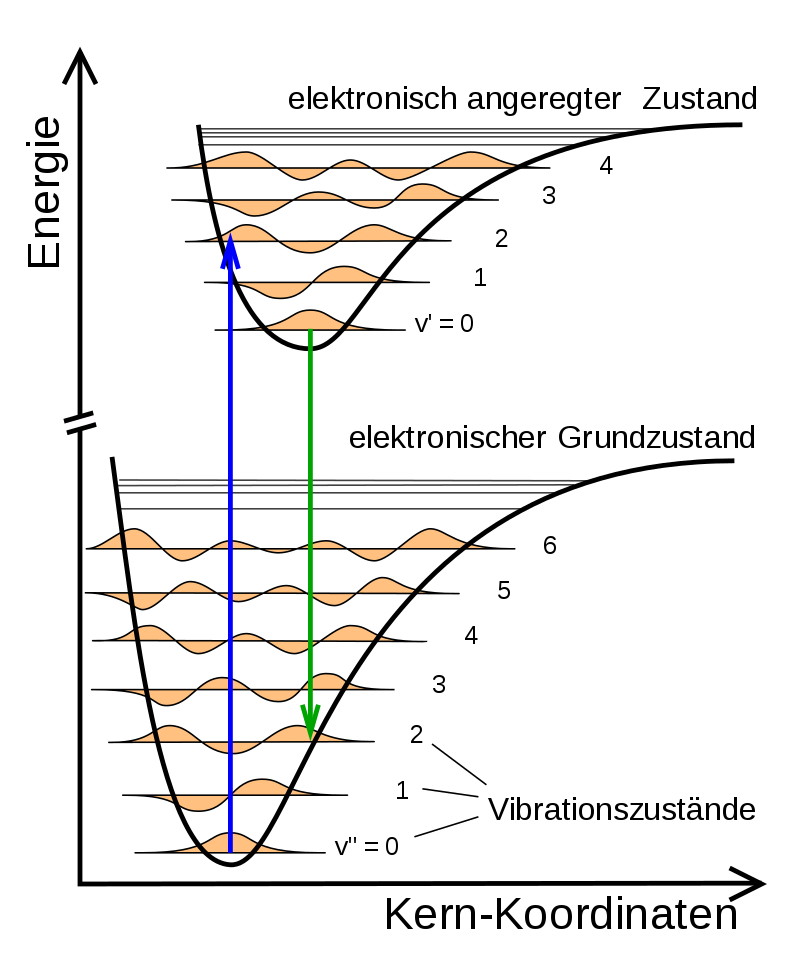
\includegraphics[width=.4\textwidth]{resources/09-05-2012/Franck-Condon-Prinzip.png}
    \caption{Schwarze Kurven: Energie eines zweiatomigen Moleküls in Abhängigkeit vom theoretisch festgehaltenen Abstand der Kerne, für zwei verschiedene Zustände der Elektronenhülle (schematisch). Die Schwingungszustände sind mit ihren Wellenfunktionen für den Kernabstand auf der Höhe der jeweiligen Energie eingezeichnet. Die beiden Pfeile stellen vibronische Übergänge dar.}
    \label{fig:q25}
\end{figure}

\paragraph{Variante 2}

Das Frank-Condon Prinzip besagt, dass elektronische Übergänge so schnell stattfinden (im Bereich von \SI{e-15}{s}), dass der Kernabstand sich effektiv nicht ändert.
Diese hohe Geschwindigkeit des elektronischen Übergangs gegenüber der Kernbewegung wird durch die geringe Masse der Elektronen ermöglicht (analog zur Born-Oppenheimer-Näherung).

Wenn ein Molekül nun von einem elektronischen Zustand in einen anderen übergeht, so ist dieser Übergang umso wahrscheinlicher, je mehr die Vibrationswellenfunktionen der beiden Zustände zueinander kompatibel sind (z. B. beim gleichen Kernabstand ein Maximum haben), siehe \autoref{fig:Condon}.

Am Beispiel der Zustände in \autoref{fig:Condon} bedeutet dies: Vom Vibrations-Grundzustand ($\nu'' = 0$) im elektronischen Grundzustand ist der wahrscheinlichste Übergang in den elektronisch angeregten Zustand derjenige, der im Vibrations-Zustand $\nu' = 2$ endet. Übergänge in andere Vibrations-Zustände können auch stattfinden, allerdings ist die Wahrscheinlichkeit dafür geringer.


\begin{figure}[H]
    \centering
    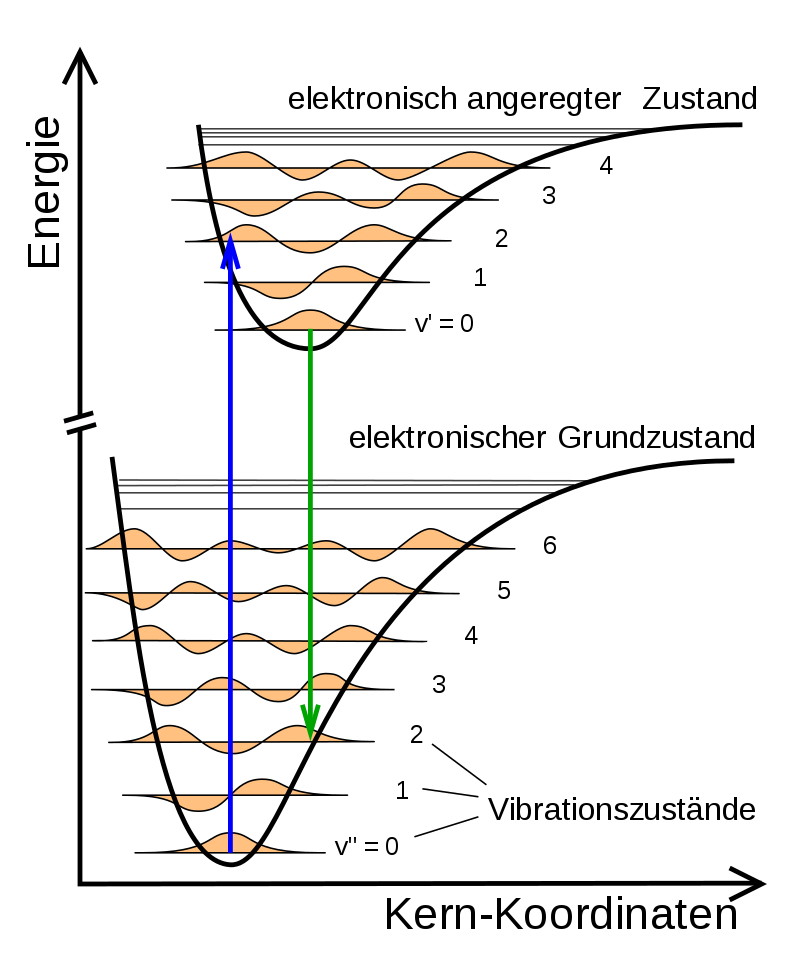
\includegraphics[width = 0.5\textwidth]{resources/09-05-2012/Franck-Condon-Prinzip}
    \caption{Schwarze Kurven Energie eines zweiatomigen Moleküls in Abhängigkeit des Abstand der Kerne, Die Pfeile symbolisieren die vibronische Übergänge.}
    \label{fig:Condon}
\end{figure}


Um so einen Übergang zu modellieren, wird ein Dipoloperator eingeführt:
\begin{equation}
    \mu = \mu_{\epsilon} + \mu_K = - e \sum_{i} \vec{r_i}  + \sum_{j} Z_j \vec{R_j} 
\end{equation}
Die Übergangswahrscheinlichkeit zwíschen den beiden Zuständen ist gegeben durch das Skalarprodukt
\begin{equation}
    P = \left\langle\psi| \mu | \psi' \right\rangle   
\end{equation}

während die Intensität I des Übergangs das Quadrat dieser Übergangswahrscheinlichkeit ist: 
\begin{equation}
    I = |P|^2
\end{equation}
Die Wellenfunktionen der beiden Zustände siehe \ref{fig:Condon} können als Produkt der elektronischen und der Vibrationswellenfunktion ausgedrückt werden.
\begin{equation}
    \psi = \psi_{\epsilon}(\vec{r_i}) \psi_v(\vec{R_j})
\end{equation} 
Da der effektive Abstand der Kerne in den Zeitskalen des Übergangs sich nicht verändert kann angenommen werden, dass die Elektron-Positionen unabhängig von den Positionen der Kerne sind.
$\langle \psi_{\epsilon}' \psi_v' | \mu_{\epsilon}| \psi_{\epsilon} \psi_v\rangle  \approx  \langle\psi_v' |\psi_v \rangle \langle\psi_{\epsilon}'|\mu_{\epsilon}| \psi_{\epsilon} \rangle $ \\
Führt man nun das Skalarprodukt aus:
\begin{equation}
    P = \langle \psi_v' | \psi_v \rangle \langle \psi_{\epsilon}' | \mu_{\epsilon} | \psi_{\epsilon} \rangle + \langle \psi_{\epsilon}' | \psi_{\epsilon} \rangle \langle\psi_v' | \mu_K |\psi_v \rangle
\end{equation}
Die zwei elektronischen Wellenfunktionen sind orthogonal aufeinander und somit ist $\langle \psi_{\epsilon}' | \psi_{\epsilon} \rangle  = 0$.
Der erste Term quadriert $|\langle \psi_v' | \psi_v \rangle|^2$ ist der Frank Condon Faktor und der zweite Term das Übergangsdipolmoment. 
Die Intensität der Schwingungsbänder wird von der Überlappung der beiden Vibrationswellenfunktionen bestimmt.
\begin{equation}
    I = |\langle \psi_v' | \psi_v \rangle \langle \psi_{\epsilon}' | \mu_{\epsilon} | \psi_{\epsilon} \rangle|^2
\end{equation}


\question{Diskutiere die Laue'sche Beugungsbedingung: anhand Ewald Konstruktion im Rahmen der Bragg'schen Interpretation.}
\label{q:26}

\textbf{Bragg'sche Streubedingung:}
\begin{align}
    n\lambda = 2 d \sin{\Theta} 
\end{align}
\textbf{Von Laue Bedingungen:}
\begin{align}
\vec{G} &= \vec{k'} - \vec{k} \\
\vec{k} \frac{1}{2} \vec{G} &= (\frac{1}{2} \vec{G})^2
\end{align}
mit den Wellenvektoren $\vec{k}$, dem reziproken Gittervektor $\vec{G}$ sowie dem Ebenenabstand $d$ und dem Streuwinkel $\Theta$ Die Bragg-Bedingung ist ein Speziallfall der Laue-Bedingung. Es elten folgende Relationen:
\begin{align}
    |\vec{G}_{h,k,l}| &= 2 |\vec{k}| \sin{\Theta} \\
    |\vec{k}| &= \frac{2 \pi}{\lambda} \\
    |\vec{G}_{h,k,l}| &= \frac{2 \pi n}{ d_{h,k,l}}
\end{align}
und somit $n \lambda = 2 d_{h,k,l}  \sin{\Theta}$. \\
Konstruktive Interferenz findet immer statt, wenn der Wellenvektor des
einfallenden Strahls an der Grenze einer Brillouin Zone liegt. Die geometrische Darstellung mit der Ewald Konstruktion unter Berücksichtigung dieser Bedingungen ermöglicht es, den Beugungswinkel $\Theta$ und den Netzebenenabstand $d$ zu bestimmen. 

\begin{figure}[H]
    \centering
    \begin{samepage}
        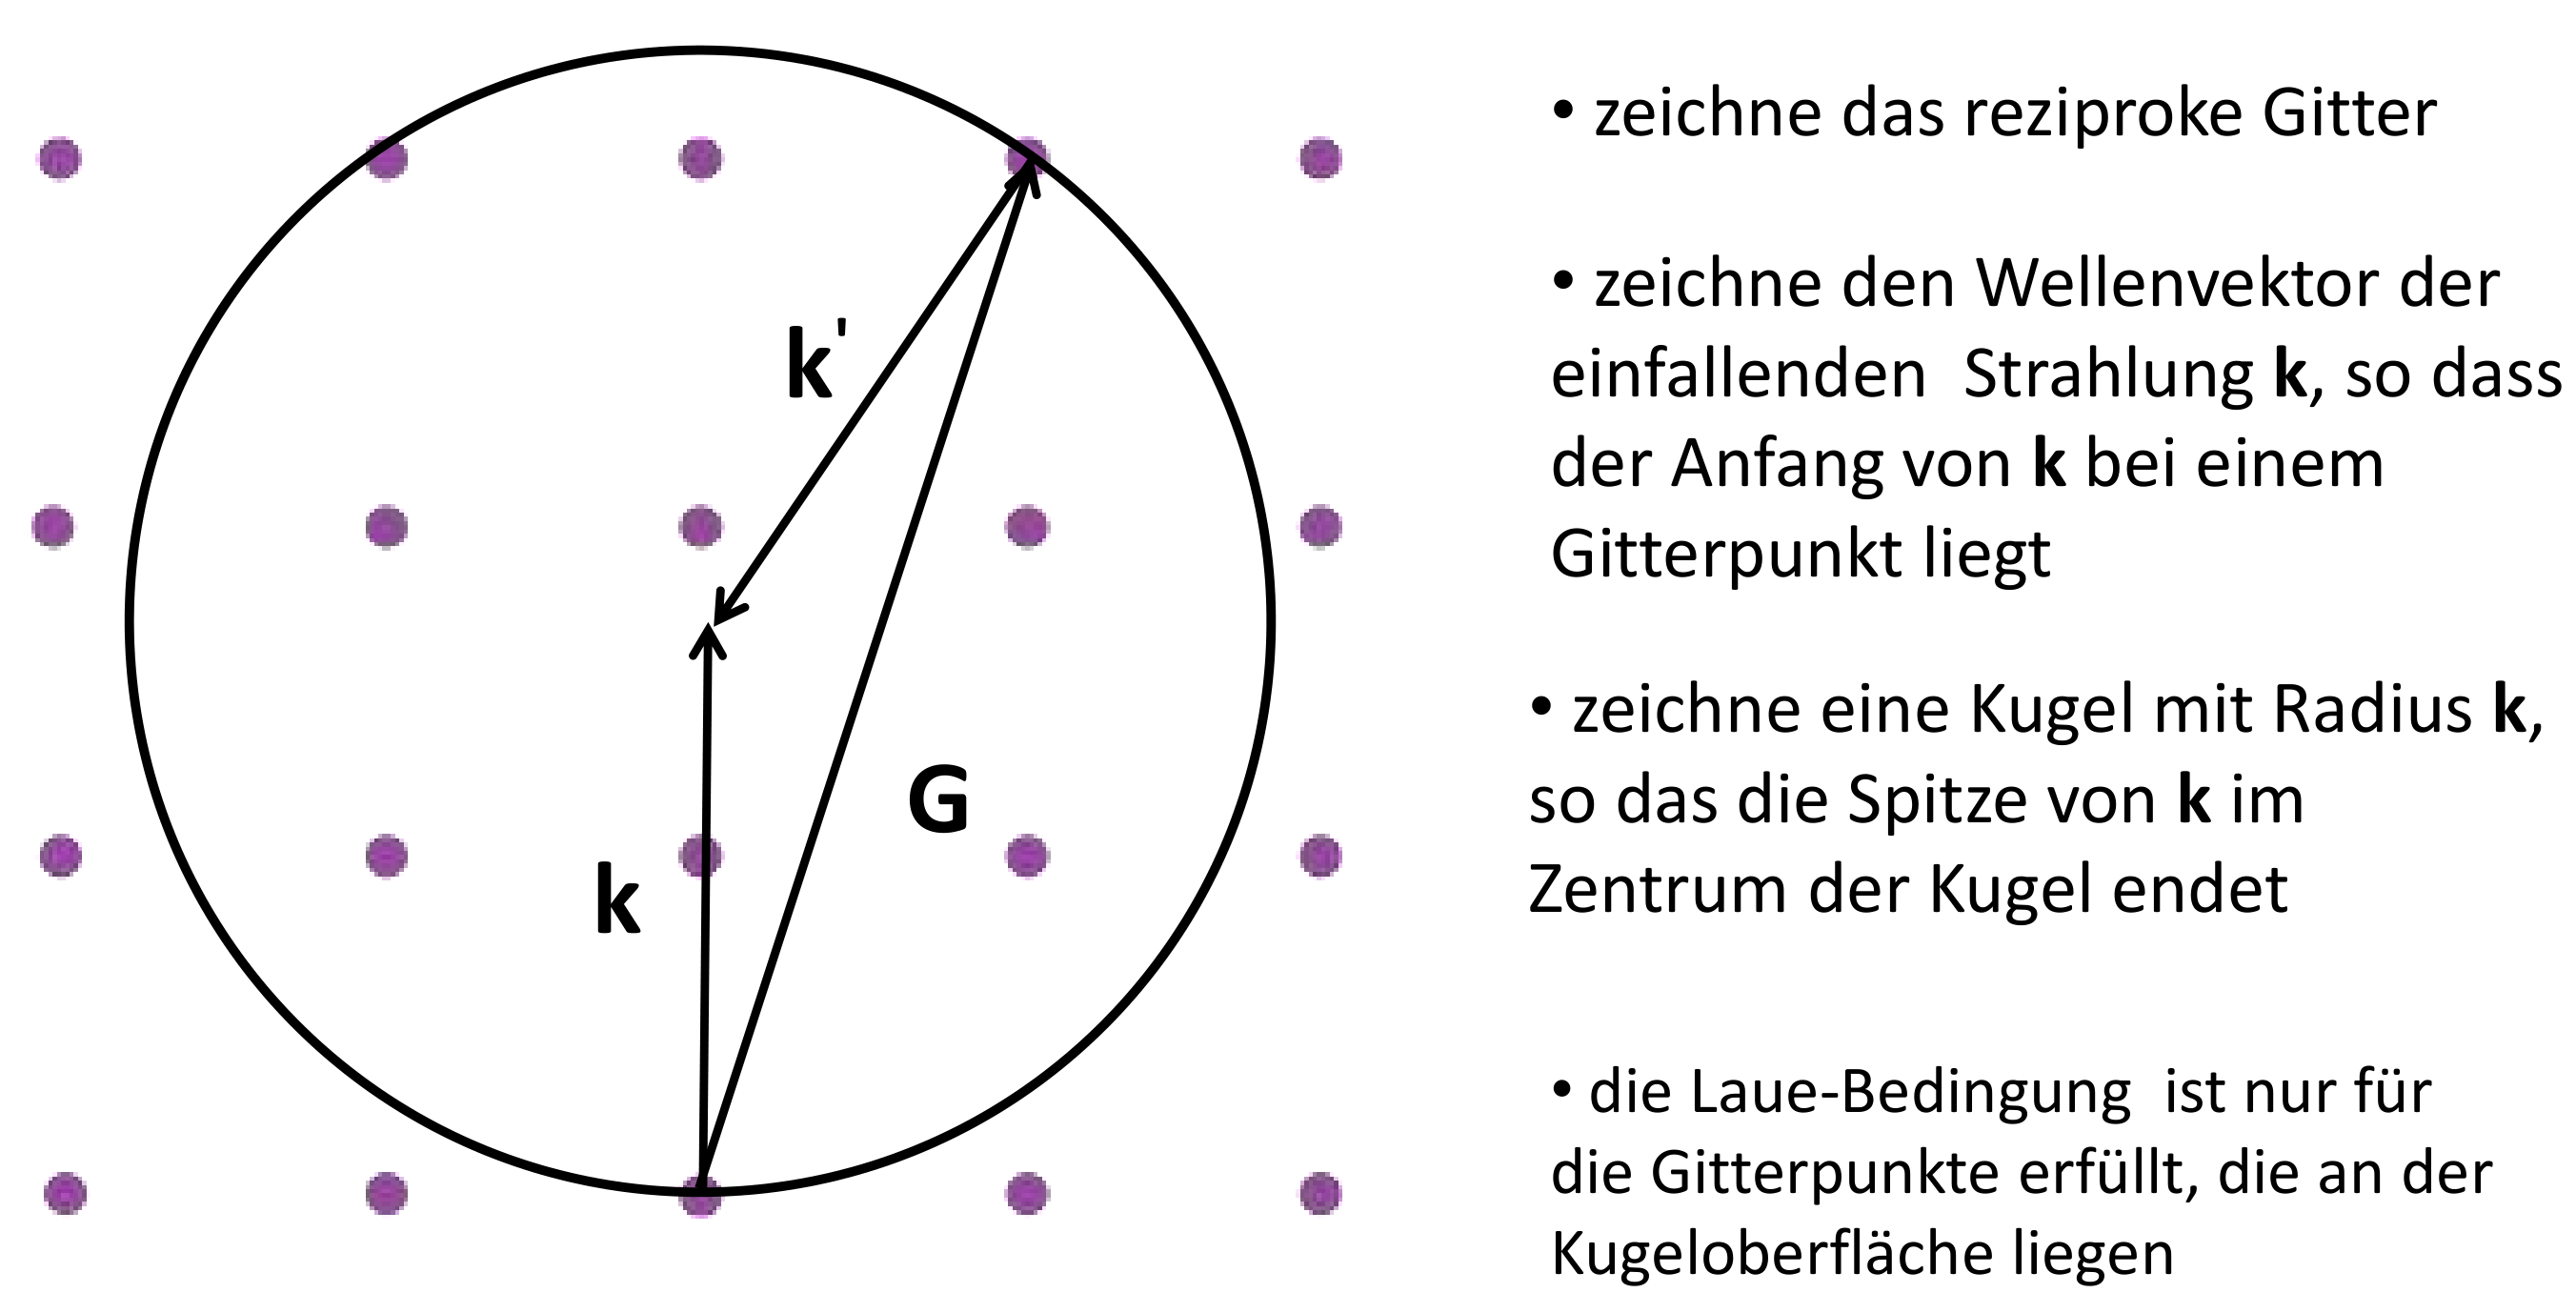
\includegraphics[width=0.8\linewidth]{resources/09-05-2012/Ewald_Konstruktion.png}
        \caption{Ewald-Konstruktion}
    \end{samepage}
\end{figure}

Die Laue-Bedingung ist hierbei nur für die Gitterpunkte erfüllt, die an der Kugeloberfläche liegen. 


\question{Erläutere den Atomfaktor und den Strukturfaktor bei der Röntgenbeugung.}
\label{q:27}

Der Strukturfaktor ist die Fourier-Transformierte $n_{\Vec{G}}$ der Elektronendichte $ n(\vec{r})$ über eine Einheitszelle. 
\begin{align}
n_{\vec{G}} = \int _{EZ} n(\vec{r}) e^{-i \vec{G} \vec{r}} d\vec{r} 
\end{align}
\begin{align}
S_{\vec{G}} = V n_{\vec{G}} 
\end{align} \medskip


\textit{(andere Definition, nicht in Surnev-Folien)} \\
Der Strukturfaktor wird aus den Formfaktoren $f_J(G)$ berechnet werden, welche ebenfalls mit Fourier-Transformation berechnet werden:
\begin{align}
f_J(G) = \int n_J(\vec{r}) e^{i \vec{G} \vec{r}} d\vec{r}
\end{align}
\begin{align}
S_{\vec{G}} = \sum_j f_j (G) e^{i \vec{G} \vec{r}_j} = \sum_j f_j e^{-2 \pi i (hx_j + ky_j + l z_j)}
\end{align}
wobei $\vec{G}_{hkl} = h\vec{b}_1+k\vec{b}_2+l\vec{b}_3$ der reziproke Gittervektor ist. \\




Der Strukturfaktor ist auch die Streuamplitude pro Einheitszelle:
\begin{align}
S_{h,k,l} = \frac{F_{h,k,l}}{N}
\end{align}
mit der Anzahl an Einheitszellen $N$ und der Streuamplitude:
\begin{align}
    F_{h,k,l} = \int n(\vec{r}) e^{-i \phi(\vec{r})} dV = \int n(\vec{r}) e^{-i \Delta \vec{k} \vec{r}} dV
\end{align}
Für diese Beschreibungen des Strukturfaktors muss die Laue-Bedingung $\vec{G} = \Delta \vec{k} = \vec{k'}-\vec{k}$ erfüllt sein. \bigskip \\

Der \textbf{Atomfaktor} (auch Streufaktor genannt) beschreibt die Beiträge eines einzelnen Atoms zur Streuung von Röntgenstrahlen bzw. das Streuvermögen der einzelnen Basisatome. Er hängt von der Atomart, der Position des Atoms im Kristallgitter und der Wellenlänge der Röntgenstrahlung ab. Der Atomfaktor ist komplex und enthält Informationen über die Elektronendichteverteilung im Atom.

Der Atomfaktor für ein Atom $j$ kann  wie folgt definiert werden:

\begin{align}
f_j = \int n_j (\vec{\rho}) e^{-i \vec{G} \vec{\rho}}
\end{align}

Mit kugelsymmetrischen $n(\vec{\rho})$ und $\vec{G} \vec{\rho} = G \rho \cos{\alpha}$ erhält man die Formel
\begin{align}
f = 4 \pi \int_0 ^{\inf} \rho^2 n(\vec{\rho}) \frac{\sin{G \rho}}{G \rho} d\rho
\end{align}

Für eine punktförmige Ladung mit $\vec{\rho} = 0$:
\begin{align}
\frac{\sin{G \rho}}{G \rho} \approx 1 \hspace{1cm} n = \frac{Z}{V} \Rightarrow f = Z
\end{align}
Für kleine Streuwinkel mit $G \approx 0$:
\begin{align}
f = Z
\end{align}

\question{Skizziere die 1. Brillouin Zone eines ebenen Rechteckgitters.}
\label{q:28}

\begin{figure}[H]
    \centering
    \begin{samepage}
        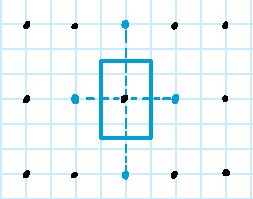
\includegraphics[width=0.4\linewidth]{resources/09-05-2012/BZ1.pdf}
        \caption[1. BZ Rechteckgitter]{1. Brillouin-Zone eines Rechteckgitters}
        \label{fig:BZ1_rechteckgitter}
    \end{samepage}
\end{figure}
\begin{enumerate}
    \item Reziprokes Gitter aufzeichnen
    \item Zellenmittelpunkt wählen
    \item Vom Mittelpunkt in beide Dimensionen den nächstgelegenen Gitterpunkt finden
    \item Mittelpunkt mit diesen Punkten verbinden
    \item Auf den Mittelpunkt der Verbindenden eine Orthogonale zeichnen
\end{enumerate}

\question{Wodurch unterscheiden sich akustische von optischen Phononen?}
\label{q:29}

Ein Phonon ist die elementare Anregung (Quant) des elastischen Feldes. Sie beschreiben die elementare bzw. kollektive Anregungen der Gitterschwingungen eines Festkörpers.
In einem dreidimensionalen Kristall mit $N$ Atomen in der primitiven Basis existieren zu jedem mit der Kristallsymmetrie verträglichen Wellenvektor 
$3N$ mögliche Schwingungsmoden:

\begin{itemize}
    \item Akustische Phononen: Diese Phononen werden auch als Schallquanten bezeichnet und sind die Quanten der Schallwellen, die sich durch das Kristallgitter fortpflanzen.
          Alle Quanten bewegen sich hier in einer Einheitszelle in Phase und haben 3 akustische Moden, wovon eine longitudinal und zwei transversal sind.

          \begin{figure}[H]
            \centering
            \begin{samepage}
                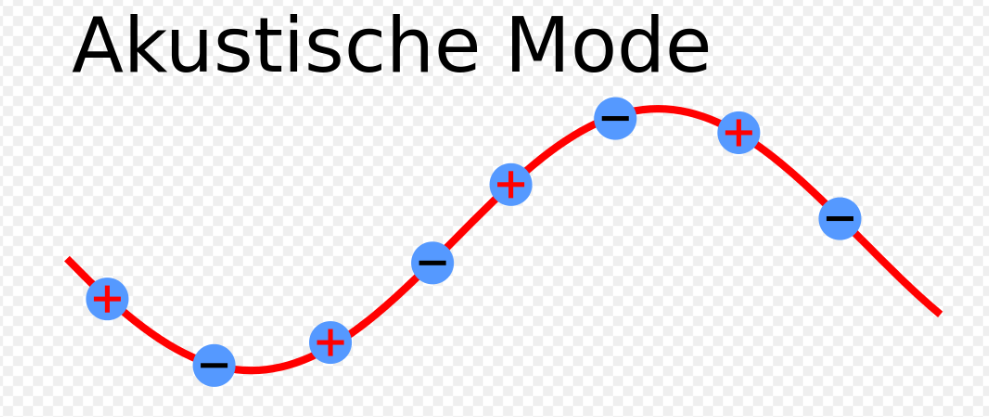
\includegraphics[width=0.8\linewidth]{resources/09-05-2012/akust.PNG}
                \caption[Akustische Transversalwellen Phononen]{Darstellung von akustischen Transversalwellen von Phononen}
                \label{fig:akustische_transversalwellen_phononen}
            \end{samepage}
          \end{figure}

    \item Optische Phononen: Diese Phononen bewegen sich in einer Basis gegenphasig, wodurch es Schwingungsmodi gibt, bei denen entgegengesetzt geladene Untergitter gegeneinander schwingen. 
          Die dabei oszillierenden Dipolmomente können mit Photonen wechselwirken. Oft kommen solche Kopplungen im Infrarotbereich, also der Wärmebewegung in Festkörpern vor.
          Beispiele für solche infrarot-aktiven Gitter sind Ionengitter wie Natriumchloridkristalle.

         \begin{figure}[H]
             \centering
             \begin{samepage}
                 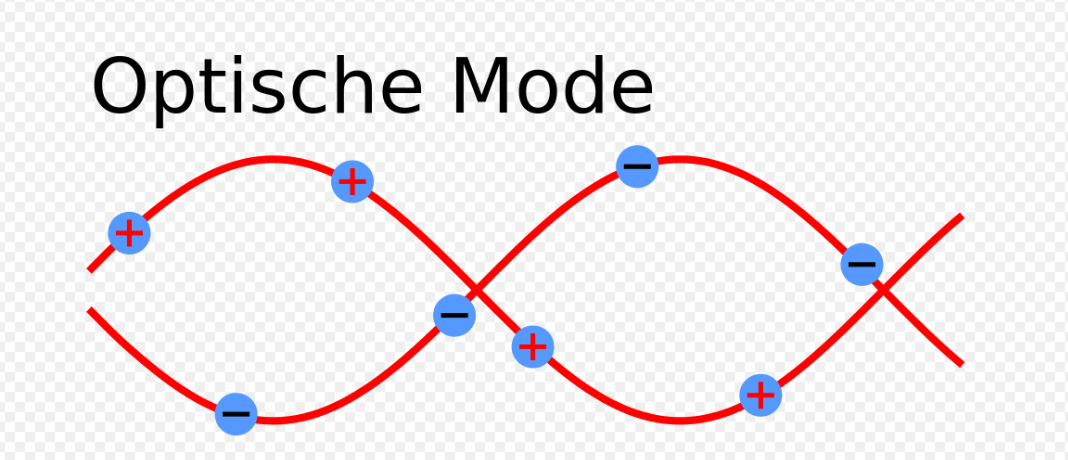
\includegraphics[width=0.8\linewidth]{resources/09-05-2012/opt.PNG}
                 \caption[Optische Wellen Phononen]{Darstellung von optischen Phononen}
                 \label{fig:optische_wellen_phononen}
             \end{samepage}
         \end{figure}

\end{itemize}



\question{Vergleiche die Einstein- und Debye-Modelle der spez. Wärme. Welche Annahme ist im 
Einstein Modell zu einfach?}
\label{q:30}

\begin{figure}[H]  
    \centering
    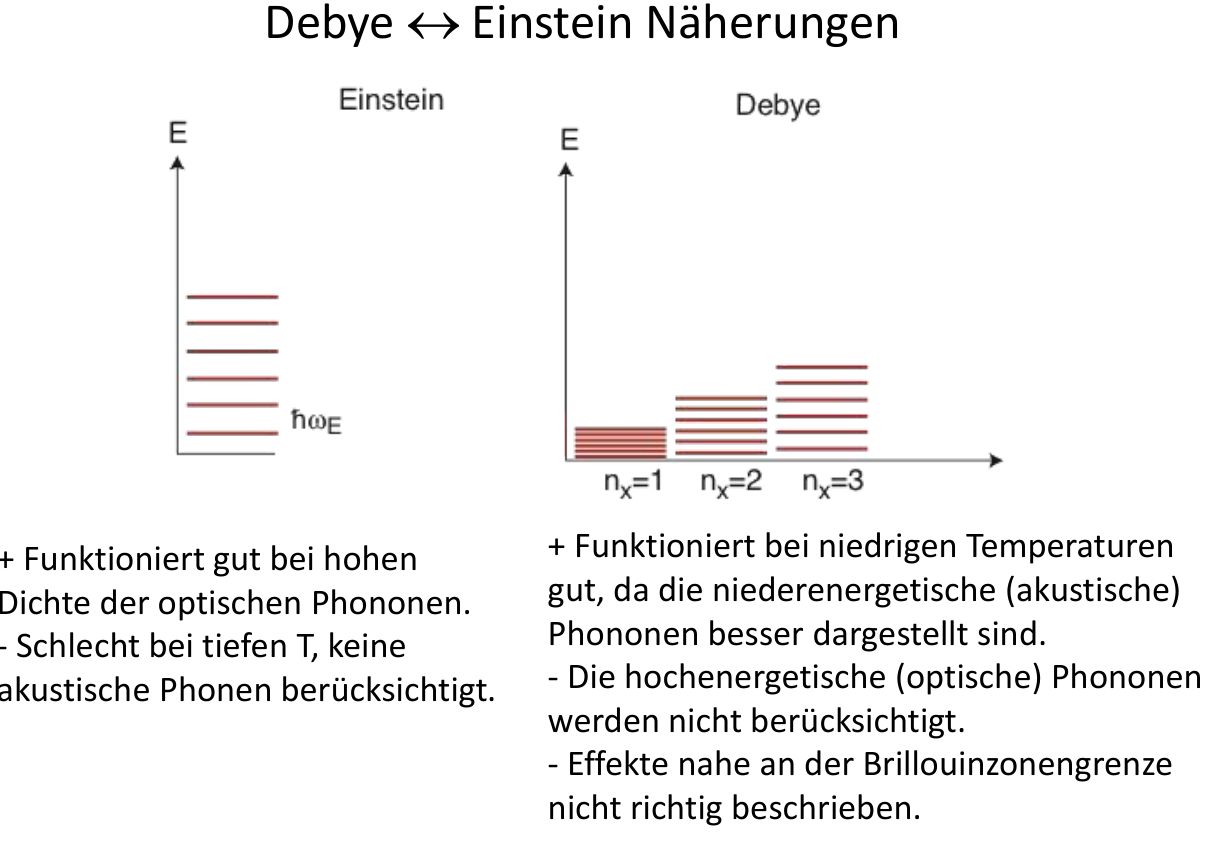
\includegraphics[width=.8\textwidth]{resources/09-05-2012/q30.png}
    \caption{Vergleich zwischen Einstein- und Debye-Modell.}
\end{figure}

Das Einsteinmodell nimmt an, dass alle Atome im Kristall mit der gleichen Frequenz schwingen, zudem werden keine akustischen Phononen berücksichtigt.

\newpage